\documentclass[1p]{elsarticle_modified}
%\bibliographystyle{elsarticle-num}

%\usepackage[colorlinks]{hyperref}
%\usepackage{abbrmath_seonhwa} %\Abb, \Ascr, \Acal ,\Abf, \Afrak
\usepackage{amsfonts}
\usepackage{amssymb}
\usepackage{amsmath}
\usepackage{amsthm}
\usepackage{scalefnt}
\usepackage{amsbsy}
\usepackage{kotex}
\usepackage{caption}
\usepackage{subfig}
\usepackage{color}
\usepackage{graphicx}
\usepackage{xcolor} %% white, black, red, green, blue, cyan, magenta, yellow
\usepackage{float}
\usepackage{setspace}
\usepackage{hyperref}

\usepackage{tikz}
\usetikzlibrary{arrows}

\usepackage{multirow}
\usepackage{array} % fixed length table
\usepackage{hhline}

%%%%%%%%%%%%%%%%%%%%%
\makeatletter
\renewcommand*\env@matrix[1][\arraystretch]{%
	\edef\arraystretch{#1}%
	\hskip -\arraycolsep
	\let\@ifnextchar\new@ifnextchar
	\array{*\c@MaxMatrixCols c}}
\makeatother %https://tex.stackexchange.com/questions/14071/how-can-i-increase-the-line-spacing-in-a-matrix
%%%%%%%%%%%%%%%

\usepackage[normalem]{ulem}

\newcommand{\msout}[1]{\ifmmode\text{\sout{\ensuremath{#1}}}\else\sout{#1}\fi}
%SOURCE: \msout is \stkout macro in https://tex.stackexchange.com/questions/20609/strikeout-in-math-mode

\newcommand{\cancel}[1]{
	\ifmmode
	{\color{red}\msout{#1}}
	\else
	{\color{red}\sout{#1}}
	\fi
}

\newcommand{\add}[1]{
	{\color{blue}\uwave{#1}}
}

\newcommand{\replace}[2]{
	\ifmmode
	{\color{red}\msout{#1}}{\color{blue}\uwave{#2}}
	\else
	{\color{red}\sout{#1}}{\color{blue}\uwave{#2}}
	\fi
}

\newcommand{\Sol}{\mathcal{S}} %segment
\newcommand{\D}{D} %diagram
\newcommand{\A}{\mathcal{A}} %arc


%%%%%%%%%%%%%%%%%%%%%%%%%%%%%5 test

\def\sl{\operatorname{\textup{SL}}(2,\Cbb)}
\def\psl{\operatorname{\textup{PSL}}(2,\Cbb)}
\def\quan{\mkern 1mu \triangleright \mkern 1mu}

\theoremstyle{definition}
\newtheorem{thm}{Theorem}[section]
\newtheorem{prop}[thm]{Proposition}
\newtheorem{lem}[thm]{Lemma}
\newtheorem{ques}[thm]{Question}
\newtheorem{cor}[thm]{Corollary}
\newtheorem{defn}[thm]{Definition}
\newtheorem{exam}[thm]{Example}
\newtheorem{rmk}[thm]{Remark}
\newtheorem{alg}[thm]{Algorithm}

\newcommand{\I}{\sqrt{-1}}
\begin{document}

%\begin{frontmatter}
%
%\title{Boundary parabolic representations of knots up to 8 crossings}
%
%%% Group authors per affiliation:
%\author{Yunhi Cho} 
%\address{Department of Mathematics, University of Seoul, Seoul, Korea}
%\ead{yhcho@uos.ac.kr}
%
%
%\author{Seonhwa Kim} %\fnref{s_kim}}
%\address{Center for Geometry and Physics, Institute for Basic Science, Pohang, 37673, Korea}
%\ead{ryeona17@ibs.re.kr}
%
%\author{Hyuk Kim}
%\address{Department of Mathematical Sciences, Seoul National University, Seoul 08826, Korea}
%\ead{hyukkim@snu.ac.kr}
%
%\author{Seokbeom Yoon}
%\address{Department of Mathematical Sciences, Seoul National University, Seoul, 08826,  Korea}
%\ead{sbyoon15@snu.ac.kr}
%
%\begin{abstract}
%We find all boundary parabolic representation of knots up to 8 crossings.
%
%\end{abstract}
%\begin{keyword}
%    \MSC[2010] 57M25 
%\end{keyword}
%
%\end{frontmatter}

%\linenumbers
%\tableofcontents
%
\newcommand\colored[1]{\textcolor{white}{\rule[-0.35ex]{0.8em}{1.4ex}}\kern-0.8em\color{red} #1}%
%\newcommand\colored[1]{\textcolor{white}{ #1}\kern-2.17ex	\textcolor{white}{ #1}\kern-1.81ex	\textcolor{white}{ #1}\kern-2.15ex\color{red}#1	}

{\Large $\underline{11a_{94}~(K11a_{94})}$}

\setlength{\tabcolsep}{10pt}
\renewcommand{\arraystretch}{1.6}
\vspace{1cm}\begin{tabular}{m{100pt}>{\centering\arraybackslash}m{274pt}}
\multirow{5}{120pt}{
	\centering
	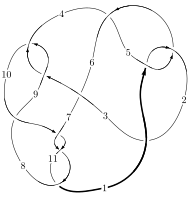
\includegraphics[width=112pt]{../../../GIT/diagram.site/Diagrams/png/343_11a_94.png}\\
\ \ \ A knot diagram\footnotemark}&
\allowdisplaybreaks
\textbf{Linearized knot diagam} \\
\cline{2-2}
 &
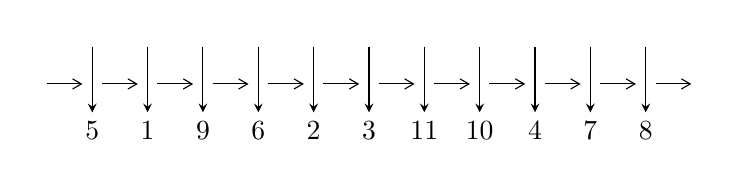
\begin{tikzpicture}[x=20pt, y=17pt]
	% nodes
	\node (C0) at (0, 0) {};
	\node (C1) at (1, 0) {};
	\node (C1U) at (1, +1) {};
	\node (C1D) at (1, -1) {5};

	\node (C2) at (2, 0) {};
	\node (C2U) at (2, +1) {};
	\node (C2D) at (2, -1) {1};

	\node (C3) at (3, 0) {};
	\node (C3U) at (3, +1) {};
	\node (C3D) at (3, -1) {9};

	\node (C4) at (4, 0) {};
	\node (C4U) at (4, +1) {};
	\node (C4D) at (4, -1) {6};

	\node (C5) at (5, 0) {};
	\node (C5U) at (5, +1) {};
	\node (C5D) at (5, -1) {2};

	\node (C6) at (6, 0) {};
	\node (C6U) at (6, +1) {};
	\node (C6D) at (6, -1) {3};

	\node (C7) at (7, 0) {};
	\node (C7U) at (7, +1) {};
	\node (C7D) at (7, -1) {11};

	\node (C8) at (8, 0) {};
	\node (C8U) at (8, +1) {};
	\node (C8D) at (8, -1) {10};

	\node (C9) at (9, 0) {};
	\node (C9U) at (9, +1) {};
	\node (C9D) at (9, -1) {4};

	\node (C10) at (10, 0) {};
	\node (C10U) at (10, +1) {};
	\node (C10D) at (10, -1) {7};

	\node (C11) at (11, 0) {};
	\node (C11U) at (11, +1) {};
	\node (C11D) at (11, -1) {8};
	\node (C12) at (12, 0) {};

	% arrows
	\draw[->,>={angle 60}]
	(C0) edge (C1) (C1) edge (C2) (C2) edge (C3) (C3) edge (C4) (C4) edge (C5) (C5) edge (C6) (C6) edge (C7) (C7) edge (C8) (C8) edge (C9) (C9) edge (C10) (C10) edge (C11) (C11) edge (C12) ;	\draw[->,>=stealth]
	(C1U) edge (C1D) (C2U) edge (C2D) (C3U) edge (C3D) (C4U) edge (C4D) (C5U) edge (C5D) (C6U) edge (C6D) (C7U) edge (C7D) (C8U) edge (C8D) (C9U) edge (C9D) (C10U) edge (C10D) (C11U) edge (C11D) ;
	\end{tikzpicture} \\
\hhline{~~} \\& 
\textbf{Solving Sequence} \\ \cline{2-2} 
 &
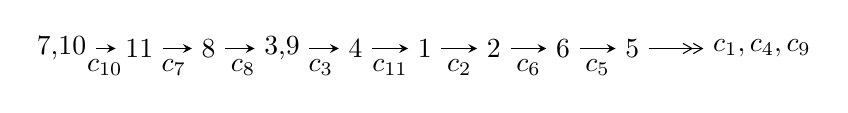
\begin{tikzpicture}[x=25pt, y=7pt]
	% node
	\node (A0) at (-1/8, 0) {7,10};
	\node (A1) at (1, 0) {11};
	\node (A2) at (2, 0) {8};
	\node (A3) at (49/16, 0) {3,9};
	\node (A4) at (33/8, 0) {4};
	\node (A5) at (41/8, 0) {1};
	\node (A6) at (49/8, 0) {2};
	\node (A7) at (57/8, 0) {6};
	\node (A8) at (65/8, 0) {5};
	\node (C1) at (1/2, -1) {$c_{10}$};
	\node (C2) at (3/2, -1) {$c_{7}$};
	\node (C3) at (5/2, -1) {$c_{8}$};
	\node (C4) at (29/8, -1) {$c_{3}$};
	\node (C5) at (37/8, -1) {$c_{11}$};
	\node (C6) at (45/8, -1) {$c_{2}$};
	\node (C7) at (53/8, -1) {$c_{6}$};
	\node (C8) at (61/8, -1) {$c_{5}$};
	\node (A9) at (10, 0) {$c_{1},c_{4},c_{9}$};

	% edge
	\draw[->,>=stealth]	
	(A0) edge (A1) (A1) edge (A2) (A2) edge (A3) (A3) edge (A4) (A4) edge (A5) (A5) edge (A6) (A6) edge (A7) (A7) edge (A8) ;
	\draw[->>,>={angle 60}]	
	(A8) edge (A9);
\end{tikzpicture} \\ 

\end{tabular} \\

\footnotetext{
The image of knot diagram is generated by the software ``\textbf{Draw programme}" developed by Andrew Bartholomew(\url{http://www.layer8.co.uk/maths/draw/index.htm\#Running-draw}), where we modified some parts for our purpose(\url{https://github.com/CATsTAILs/LinksPainter}).
}\phantom \\ \newline 
\centering \textbf{Ideals for irreducible components\footnotemark of $X_{\text{par}}$} 
 
\begin{align*}
I^u_{1}&=\langle 
-17 u^{55}+43 u^{54}+\cdots+2 b-11,\;-3 u^{55}+7 u^{54}+\cdots+4 a+3,\;u^{56}-4 u^{55}+\cdots-2 u-1\rangle \\
I^u_{2}&=\langle 
b,\;a^3+a^2+2 a+1,\;u+1\rangle \\
\\
\end{align*}
\raggedright * 2 irreducible components of $\dim_{\mathbb{C}}=0$, with total 59 representations.\\
\footnotetext{All coefficients of polynomials are rational numbers. But the coefficients are sometimes approximated in decimal forms when there is not enough margin.}
\newpage
\renewcommand{\arraystretch}{1}
\centering \section*{I. $I^u_{1}= \langle -17 u^{55}+43 u^{54}+\cdots+2 b-11,\;-3 u^{55}+7 u^{54}+\cdots+4 a+3,\;u^{56}-4 u^{55}+\cdots-2 u-1 \rangle$}
\flushleft \textbf{(i) Arc colorings}\\
\begin{tabular}{m{7pt} m{180pt} m{7pt} m{180pt} }
\flushright $a_{7}=$&$\begin{pmatrix}0\\u\end{pmatrix}$ \\
\flushright $a_{10}=$&$\begin{pmatrix}1\\0\end{pmatrix}$ \\
\flushright $a_{11}=$&$\begin{pmatrix}1\\u^2\end{pmatrix}$ \\
\flushright $a_{8}=$&$\begin{pmatrix}- u\\- u^3+u\end{pmatrix}$ \\
\flushright $a_{3}=$&$\begin{pmatrix}\frac{3}{4} u^{55}-\frac{7}{4} u^{54}+\cdots+\frac{13}{4} u-\frac{3}{4}\\\frac{17}{2} u^{55}-\frac{43}{2} u^{54}+\cdots+\frac{31}{2} u+\frac{11}{2}\end{pmatrix}$ \\
\flushright $a_{9}=$&$\begin{pmatrix}u^3-2 u\\- u^3+u\end{pmatrix}$ \\
\flushright $a_{4}=$&$\begin{pmatrix}\frac{33}{4} u^{55}-\frac{85}{4} u^{54}+\cdots+\frac{71}{4} u+\frac{19}{4}\\\frac{5}{2} u^{55}-\frac{17}{2} u^{54}+\cdots+\frac{17}{2} u+\frac{5}{2}\end{pmatrix}$ \\
\flushright $a_{1}=$&$\begin{pmatrix}- u^2+1\\- u^4+2 u^2\end{pmatrix}$ \\
\flushright $a_{2}=$&$\begin{pmatrix}\frac{27}{4} u^{55}-\frac{71}{4} u^{54}+\cdots+\frac{57}{4} u+\frac{13}{4}\\\frac{27}{4} u^{55}-\frac{75}{4} u^{54}+\cdots+\frac{61}{4} u+\frac{21}{4}\end{pmatrix}$ \\
\flushright $a_{6}=$&$\begin{pmatrix}\frac{1}{4} u^{55}-\frac{3}{4} u^{54}+\cdots-\frac{13}{4} u-\frac{3}{4}\\- u^{10}+4 u^8+2 u^7-5 u^6-6 u^5+4 u^3+3 u^2+2 u\end{pmatrix}$ \\
\flushright $a_{5}=$&$\begin{pmatrix}4 u^{55}-\frac{23}{2} u^{54}+\cdots+5 u+\frac{3}{2}\\-\frac{9}{4} u^{55}+\frac{25}{4} u^{54}+\cdots-\frac{7}{4} u-\frac{7}{4}\end{pmatrix}$\\ \flushright $a_{5}=$&$\begin{pmatrix}4 u^{55}-\frac{23}{2} u^{54}+\cdots+5 u+\frac{3}{2}\\-\frac{9}{4} u^{55}+\frac{25}{4} u^{54}+\cdots-\frac{7}{4} u-\frac{7}{4}\end{pmatrix}$\\&\end{tabular}
\flushleft \textbf{(ii) Obstruction class $= -1$}\\~\\
\flushleft \textbf{(iii) Cusp Shapes $= -2 u^{55}+\frac{15}{2} u^{54}+\cdots+5 u-\frac{29}{2}$}\\~\\
\newpage\renewcommand{\arraystretch}{1}
\flushleft \textbf{(iv) u-Polynomials at the component}\newline \\
\begin{tabular}{m{50pt}|m{274pt}}
Crossings & \hspace{64pt}u-Polynomials at each crossing \\
\hline $$\begin{aligned}c_{1},c_{5}\end{aligned}$$&$\begin{aligned}
&u^{56}+2 u^{55}+\cdots-5 u-1
\end{aligned}$\\
\hline $$\begin{aligned}c_{2},c_{4}\end{aligned}$$&$\begin{aligned}
&u^{56}+18 u^{55}+\cdots+5 u+1
\end{aligned}$\\
\hline $$\begin{aligned}c_{3},c_{9}\end{aligned}$$&$\begin{aligned}
&u^{56}- u^{55}+\cdots+12 u+8
\end{aligned}$\\
\hline $$\begin{aligned}c_{6}\end{aligned}$$&$\begin{aligned}
&u^{56}-2 u^{55}+\cdots-145 u-25
\end{aligned}$\\
\hline $$\begin{aligned}c_{7},c_{10},c_{11}\end{aligned}$$&$\begin{aligned}
&u^{56}-4 u^{55}+\cdots-2 u-1
\end{aligned}$\\
\hline $$\begin{aligned}c_{8}\end{aligned}$$&$\begin{aligned}
&u^{56}+21 u^{55}+\cdots+592 u+64
\end{aligned}$\\
\hline
\end{tabular}\\~\\
\newpage\renewcommand{\arraystretch}{1}
\flushleft \textbf{(v) Riley Polynomials at the component}\newline \\
\begin{tabular}{m{50pt}|m{274pt}}
Crossings & \hspace{64pt}Riley Polynomials at each crossing \\
\hline $$\begin{aligned}c_{1},c_{5}\end{aligned}$$&$\begin{aligned}
&y^{56}-18 y^{55}+\cdots-5 y+1
\end{aligned}$\\
\hline $$\begin{aligned}c_{2},c_{4}\end{aligned}$$&$\begin{aligned}
&y^{56}+42 y^{55}+\cdots-77 y+1
\end{aligned}$\\
\hline $$\begin{aligned}c_{3},c_{9}\end{aligned}$$&$\begin{aligned}
&y^{56}-21 y^{55}+\cdots-592 y+64
\end{aligned}$\\
\hline $$\begin{aligned}c_{6}\end{aligned}$$&$\begin{aligned}
&y^{56}+6 y^{55}+\cdots+7275 y+625
\end{aligned}$\\
\hline $$\begin{aligned}c_{7},c_{10},c_{11}\end{aligned}$$&$\begin{aligned}
&y^{56}-48 y^{55}+\cdots-18 y+1
\end{aligned}$\\
\hline $$\begin{aligned}c_{8}\end{aligned}$$&$\begin{aligned}
&y^{56}+23 y^{55}+\cdots-85248 y+4096
\end{aligned}$\\
\hline
\end{tabular}\\~\\
\newpage\flushleft \textbf{(vi) Complex Volumes and Cusp Shapes}
$$\begin{array}{c|c|c}  
\text{Solutions to }I^u_{1}& \I (\text{vol} + \sqrt{-1}CS) & \text{Cusp shape}\\
 \hline 
\begin{aligned}
u &= -0.866172 + 0.412104 I \\
a &= \phantom{-}0.716759 + 0.563360 I \\
b &= \phantom{-}0.408158 - 0.290046 I\end{aligned}
 & -3.84915 - 0.47402 I & -20.0517 + 1.8006 I \\ \hline\begin{aligned}
u &= -0.866172 - 0.412104 I \\
a &= \phantom{-}0.716759 - 0.563360 I \\
b &= \phantom{-}0.408158 + 0.290046 I\end{aligned}
 & -3.84915 + 0.47402 I & -20.0517 - 1.8006 I \\ \hline\begin{aligned}
u &= -0.188462 + 0.854305 I \\
a &= \phantom{-}1.56928 + 1.20703 I \\
b &= -1.35361 - 1.14786 I\end{aligned}
 & \phantom{-}3.70616 + 10.08220 I & -9.08620 - 8.29722 I \\ \hline\begin{aligned}
u &= -0.188462 - 0.854305 I \\
a &= \phantom{-}1.56928 - 1.20703 I \\
b &= -1.35361 + 1.14786 I\end{aligned}
 & \phantom{-}3.70616 - 10.08220 I & -9.08620 + 8.29722 I \\ \hline\begin{aligned}
u &= -0.165662 + 0.838312 I \\
a &= -1.65426 - 0.98689 I \\
b &= \phantom{-}1.41656 + 1.00950 I\end{aligned}
 & \phantom{-}4.58143 + 4.28016 I & -7.26827 - 3.33660 I \\ \hline\begin{aligned}
u &= -0.165662 - 0.838312 I \\
a &= -1.65426 + 0.98689 I \\
b &= \phantom{-}1.41656 - 1.00950 I\end{aligned}
 & \phantom{-}4.58143 - 4.28016 I & -7.26827 + 3.33660 I \\ \hline\begin{aligned}
u &= -1.050040 + 0.463708 I \\
a &= \phantom{-}0.479637 + 1.195890 I \\
b &= \phantom{-}0.907676 - 0.666506 I\end{aligned}
 & \phantom{-}1.07406 - 5.37584 I & \phantom{-0.000000 } 0 \\ \hline\begin{aligned}
u &= -1.050040 - 0.463708 I \\
a &= \phantom{-}0.479637 - 1.195890 I \\
b &= \phantom{-}0.907676 + 0.666506 I\end{aligned}
 & \phantom{-}1.07406 + 5.37584 I & \phantom{-0.000000 } 0 \\ \hline\begin{aligned}
u &= -1.078200 + 0.427394 I \\
a &= -0.272195 - 1.149050 I \\
b &= -1.066620 + 0.514728 I\end{aligned}
 & \phantom{-}1.79919 + 0.26900 I & \phantom{-0.000000 } 0 \\ \hline\begin{aligned}
u &= -1.078200 - 0.427394 I \\
a &= -0.272195 + 1.149050 I \\
b &= -1.066620 - 0.514728 I\end{aligned}
 & \phantom{-}1.79919 - 0.26900 I & \phantom{-0.000000 } 0\\
 \hline 
 \end{array}$$\newpage$$\begin{array}{c|c|c}  
\text{Solutions to }I^u_{1}& \I (\text{vol} + \sqrt{-1}CS) & \text{Cusp shape}\\
 \hline 
\begin{aligned}
u &= -0.617027 + 0.535939 I \\
a &= \phantom{-}0.858761 - 0.032635 I \\
b &= \phantom{-}0.0856353 + 0.0708847 I\end{aligned}
 & -0.71189 + 4.42421 I & -14.7302 - 6.6620 I \\ \hline\begin{aligned}
u &= -0.617027 - 0.535939 I \\
a &= \phantom{-}0.858761 + 0.032635 I \\
b &= \phantom{-}0.0856353 - 0.0708847 I\end{aligned}
 & -0.71189 - 4.42421 I & -14.7302 + 6.6620 I \\ \hline\begin{aligned}
u &= -1.168010 + 0.209136 I \\
a &= \phantom{-}0.247139 - 0.431048 I \\
b &= -1.026800 - 0.591291 I\end{aligned}
 & -1.37028 + 0.97595 I & \phantom{-0.000000 } 0 \\ \hline\begin{aligned}
u &= -1.168010 - 0.209136 I \\
a &= \phantom{-}0.247139 + 0.431048 I \\
b &= -1.026800 + 0.591291 I\end{aligned}
 & -1.37028 - 0.97595 I & \phantom{-0.000000 } 0 \\ \hline\begin{aligned}
u &= -0.241002 + 0.768489 I \\
a &= \phantom{-}0.882963 + 0.837698 I \\
b &= -0.943312 - 0.875499 I\end{aligned}
 & -1.88523 + 4.71954 I & -14.7264 - 6.6425 I \\ \hline\begin{aligned}
u &= -0.241002 - 0.768489 I \\
a &= \phantom{-}0.882963 - 0.837698 I \\
b &= -0.943312 + 0.875499 I\end{aligned}
 & -1.88523 - 4.71954 I & -14.7264 + 6.6425 I \\ \hline\begin{aligned}
u &= \phantom{-}1.225830 + 0.232995 I \\
a &= \phantom{-}0.37066 - 1.43650 I \\
b &= \phantom{-}0.872612 - 0.365716 I\end{aligned}
 & \phantom{-}1.47062 + 1.23708 I & \phantom{-0.000000 } 0 \\ \hline\begin{aligned}
u &= \phantom{-}1.225830 - 0.232995 I \\
a &= \phantom{-}0.37066 + 1.43650 I \\
b &= \phantom{-}0.872612 + 0.365716 I\end{aligned}
 & \phantom{-}1.47062 - 1.23708 I & \phantom{-0.000000 } 0 \\ \hline\begin{aligned}
u &= \phantom{-}1.240870 + 0.261920 I \\
a &= -0.09120 + 1.42966 I \\
b &= -1.006580 + 0.465327 I\end{aligned}
 & \phantom{-}1.86713 - 4.74693 I & \phantom{-0.000000 } 0 \\ \hline\begin{aligned}
u &= \phantom{-}1.240870 - 0.261920 I \\
a &= -0.09120 - 1.42966 I \\
b &= -1.006580 - 0.465327 I\end{aligned}
 & \phantom{-}1.86713 + 4.74693 I & \phantom{-0.000000 } 0\\
 \hline 
 \end{array}$$\newpage$$\begin{array}{c|c|c}  
\text{Solutions to }I^u_{1}& \I (\text{vol} + \sqrt{-1}CS) & \text{Cusp shape}\\
 \hline 
\begin{aligned}
u &= -0.140644 + 0.703431 I \\
a &= -1.178460 - 0.095442 I \\
b &= \phantom{-}1.155670 + 0.456832 I\end{aligned}
 & \phantom{-}1.60637 + 2.37356 I & -6.13877 - 4.17137 I \\ \hline\begin{aligned}
u &= -0.140644 - 0.703431 I \\
a &= -1.178460 + 0.095442 I \\
b &= \phantom{-}1.155670 - 0.456832 I\end{aligned}
 & \phantom{-}1.60637 - 2.37356 I & -6.13877 + 4.17137 I \\ \hline\begin{aligned}
u &= \phantom{-}0.048164 + 0.710249 I \\
a &= -2.01204 + 0.89303 I \\
b &= \phantom{-}1.59325 - 0.13231 I\end{aligned}
 & \phantom{-}5.50599 + 1.24032 I & -5.23066 - 2.33484 I \\ \hline\begin{aligned}
u &= \phantom{-}0.048164 - 0.710249 I \\
a &= -2.01204 - 0.89303 I \\
b &= \phantom{-}1.59325 + 0.13231 I\end{aligned}
 & \phantom{-}5.50599 - 1.24032 I & -5.23066 + 2.33484 I \\ \hline\begin{aligned}
u &= -0.448607 + 0.542572 I \\
a &= -0.438992 + 0.149521 I \\
b &= -0.297929 - 0.283370 I\end{aligned}
 & -0.279032 - 0.387064 I & -13.17728 - 1.08778 I \\ \hline\begin{aligned}
u &= -0.448607 - 0.542572 I \\
a &= -0.438992 - 0.149521 I \\
b &= -0.297929 + 0.283370 I\end{aligned}
 & -0.279032 + 0.387064 I & -13.17728 + 1.08778 I \\ \hline\begin{aligned}
u &= \phantom{-}0.086804 + 0.689503 I \\
a &= \phantom{-}2.00700 - 1.20329 I \\
b &= -1.55835 + 0.31132 I\end{aligned}
 & \phantom{-}4.89165 - 4.55526 I & -6.35177 + 3.19659 I \\ \hline\begin{aligned}
u &= \phantom{-}0.086804 - 0.689503 I \\
a &= \phantom{-}2.00700 + 1.20329 I \\
b &= -1.55835 - 0.31132 I\end{aligned}
 & \phantom{-}4.89165 + 4.55526 I & -6.35177 - 3.19659 I \\ \hline\begin{aligned}
u &= -1.305330 + 0.049118 I \\
a &= -0.193950 - 0.243423 I \\
b &= \phantom{-}0.39449 + 1.81061 I\end{aligned}
 & -2.36775 - 2.29859 I & \phantom{-0.000000 } 0 \\ \hline\begin{aligned}
u &= -1.305330 - 0.049118 I \\
a &= -0.193950 + 0.243423 I \\
b &= \phantom{-}0.39449 - 1.81061 I\end{aligned}
 & -2.36775 + 2.29859 I & \phantom{-0.000000 } 0\\
 \hline 
 \end{array}$$\newpage$$\begin{array}{c|c|c}  
\text{Solutions to }I^u_{1}& \I (\text{vol} + \sqrt{-1}CS) & \text{Cusp shape}\\
 \hline 
\begin{aligned}
u &= -1.302410 + 0.198734 I \\
a &= -0.712631 + 0.159499 I \\
b &= \phantom{-}1.50723 + 1.35120 I\end{aligned}
 & -4.77983 + 2.82843 I & \phantom{-0.000000 } 0 \\ \hline\begin{aligned}
u &= -1.302410 - 0.198734 I \\
a &= -0.712631 - 0.159499 I \\
b &= \phantom{-}1.50723 - 1.35120 I\end{aligned}
 & -4.77983 - 2.82843 I & \phantom{-0.000000 } 0 \\ \hline\begin{aligned}
u &= -1.296500 + 0.293943 I \\
a &= \phantom{-}0.904976 - 0.648287 I \\
b &= -2.05274 - 0.77370 I\end{aligned}
 & \phantom{-}1.30531 + 2.39964 I & \phantom{-0.000000 } 0 \\ \hline\begin{aligned}
u &= -1.296500 - 0.293943 I \\
a &= \phantom{-}0.904976 + 0.648287 I \\
b &= -2.05274 + 0.77370 I\end{aligned}
 & \phantom{-}1.30531 - 2.39964 I & \phantom{-0.000000 } 0 \\ \hline\begin{aligned}
u &= -1.322480 + 0.285611 I \\
a &= -1.042770 + 0.548589 I \\
b &= \phantom{-}2.18268 + 0.97725 I\end{aligned}
 & \phantom{-}0.45930 + 8.10035 I & \phantom{-0.000000 } 0 \\ \hline\begin{aligned}
u &= -1.322480 - 0.285611 I \\
a &= -1.042770 - 0.548589 I \\
b &= \phantom{-}2.18268 - 0.97725 I\end{aligned}
 & \phantom{-}0.45930 - 8.10035 I & \phantom{-0.000000 } 0 \\ \hline\begin{aligned}
u &= \phantom{-}1.350790 + 0.293586 I \\
a &= \phantom{-}0.501547 + 0.644493 I \\
b &= -1.03042 + 1.22757 I\end{aligned}
 & -3.10733 - 6.00225 I & \phantom{-0.000000 } 0 \\ \hline\begin{aligned}
u &= \phantom{-}1.350790 - 0.293586 I \\
a &= \phantom{-}0.501547 - 0.644493 I \\
b &= -1.03042 - 1.22757 I\end{aligned}
 & -3.10733 + 6.00225 I & \phantom{-0.000000 } 0 \\ \hline\begin{aligned}
u &= \phantom{-}1.372070 + 0.235523 I \\
a &= -0.076585 - 0.360451 I \\
b &= \phantom{-}0.548336 - 1.187110 I\end{aligned}
 & -5.59879 - 2.28336 I & \phantom{-0.000000 } 0 \\ \hline\begin{aligned}
u &= \phantom{-}1.372070 - 0.235523 I \\
a &= -0.076585 + 0.360451 I \\
b &= \phantom{-}0.548336 + 1.187110 I\end{aligned}
 & -5.59879 + 2.28336 I & \phantom{-0.000000 } 0\\
 \hline 
 \end{array}$$\newpage$$\begin{array}{c|c|c}  
\text{Solutions to }I^u_{1}& \I (\text{vol} + \sqrt{-1}CS) & \text{Cusp shape}\\
 \hline 
\begin{aligned}
u &= \phantom{-}1.403150 + 0.062138 I \\
a &= \phantom{-}0.772974 - 0.030882 I \\
b &= -0.360419 - 0.400109 I\end{aligned}
 & -6.13819 - 1.16533 I & \phantom{-0.000000 } 0 \\ \hline\begin{aligned}
u &= \phantom{-}1.403150 - 0.062138 I \\
a &= \phantom{-}0.772974 + 0.030882 I \\
b &= -0.360419 + 0.400109 I\end{aligned}
 & -6.13819 + 1.16533 I & \phantom{-0.000000 } 0 \\ \hline\begin{aligned}
u &= \phantom{-}1.37282 + 0.35653 I \\
a &= \phantom{-}1.134610 + 0.597959 I \\
b &= -1.51941 + 1.55952 I\end{aligned}
 & -0.27805 - 8.58003 I & \phantom{-0.000000 } 0 \\ \hline\begin{aligned}
u &= \phantom{-}1.37282 - 0.35653 I \\
a &= \phantom{-}1.134610 - 0.597959 I \\
b &= -1.51941 - 1.55952 I\end{aligned}
 & -0.27805 + 8.58003 I & \phantom{-0.000000 } 0 \\ \hline\begin{aligned}
u &= \phantom{-}1.39495 + 0.31342 I \\
a &= -0.767957 - 0.290710 I \\
b &= \phantom{-}1.06397 - 1.65056 I\end{aligned}
 & -7.07159 - 8.63297 I & \phantom{-0.000000 } 0 \\ \hline\begin{aligned}
u &= \phantom{-}1.39495 - 0.31342 I \\
a &= -0.767957 + 0.290710 I \\
b &= \phantom{-}1.06397 + 1.65056 I\end{aligned}
 & -7.07159 + 8.63297 I & \phantom{-0.000000 } 0 \\ \hline\begin{aligned}
u &= \phantom{-}1.38707 + 0.36194 I \\
a &= -1.225820 - 0.469271 I \\
b &= \phantom{-}1.54315 - 1.70908 I\end{aligned}
 & -1.2781 - 14.4580 I & \phantom{-0.000000 } 0 \\ \hline\begin{aligned}
u &= \phantom{-}1.38707 - 0.36194 I \\
a &= -1.225820 + 0.469271 I \\
b &= \phantom{-}1.54315 + 1.70908 I\end{aligned}
 & -1.2781 + 14.4580 I & \phantom{-0.000000 } 0 \\ \hline\begin{aligned}
u &= \phantom{-}1.45135 + 0.08180 I \\
a &= -0.739121 - 0.103503 I \\
b &= \phantom{-}0.656296 + 0.649639 I\end{aligned}
 & -7.50796 - 6.20957 I & \phantom{-0.000000 } 0 \\ \hline\begin{aligned}
u &= \phantom{-}1.45135 - 0.08180 I \\
a &= -0.739121 + 0.103503 I \\
b &= \phantom{-}0.656296 - 0.649639 I\end{aligned}
 & -7.50796 + 6.20957 I & \phantom{-0.000000 } 0\\
 \hline 
 \end{array}$$\newpage$$\begin{array}{c|c|c}  
\text{Solutions to }I^u_{1}& \I (\text{vol} + \sqrt{-1}CS) & \text{Cusp shape}\\
 \hline 
\begin{aligned}
u &= \phantom{-}1.45795\phantom{ +0.000000I} \\
a &= -0.872262\phantom{ +0.000000I} \\
b &= \phantom{-}0.821275\phantom{ +0.000000I}\end{aligned}
 & -11.3625\phantom{ +0.000000I} & \phantom{-0.000000 } 0 \\ \hline\begin{aligned}
u &= -0.035406 + 0.444835 I \\
a &= \phantom{-}0.396342 - 1.248670 I \\
b &= -0.772381 + 0.172570 I\end{aligned}
 & -0.691494 - 0.342390 I & -11.27142 + 0.66679 I \\ \hline\begin{aligned}
u &= -0.035406 - 0.444835 I \\
a &= \phantom{-}0.396342 + 1.248670 I \\
b &= -0.772381 - 0.172570 I\end{aligned}
 & -0.691494 + 0.342390 I & -11.27142 - 0.66679 I \\ \hline\begin{aligned}
u &= \phantom{-}0.316601 + 0.055324 I \\
a &= \phantom{-}0.04721 - 3.30384 I \\
b &= -0.067426 + 0.690981 I\end{aligned}
 & \phantom{-}2.47292 + 2.72146 I & -4.00548 - 3.04642 I \\ \hline\begin{aligned}
u &= \phantom{-}0.316601 - 0.055324 I \\
a &= \phantom{-}0.04721 + 3.30384 I \\
b &= -0.067426 - 0.690981 I\end{aligned}
 & \phantom{-}2.47292 - 2.72146 I & -4.00548 + 3.04642 I \\ \hline\begin{aligned}
u &= -0.306961\phantom{ +0.000000I} \\
a &= -1.09551\phantom{ +0.000000I} \\
b &= -0.380686\phantom{ +0.000000I}\end{aligned}
 & -0.701749\phantom{ +0.000000I} & -14.3130\phantom{ +0.000000I}\\
 \hline 
 \end{array}$$\newpage\newpage\renewcommand{\arraystretch}{1}
\centering \section*{II. $I^u_{2}= \langle b,\;a^3+a^2+2 a+1,\;u+1 \rangle$}
\flushleft \textbf{(i) Arc colorings}\\
\begin{tabular}{m{7pt} m{180pt} m{7pt} m{180pt} }
\flushright $a_{7}=$&$\begin{pmatrix}0\\-1\end{pmatrix}$ \\
\flushright $a_{10}=$&$\begin{pmatrix}1\\0\end{pmatrix}$ \\
\flushright $a_{11}=$&$\begin{pmatrix}1\\1\end{pmatrix}$ \\
\flushright $a_{8}=$&$\begin{pmatrix}1\\0\end{pmatrix}$ \\
\flushright $a_{3}=$&$\begin{pmatrix}a\\0\end{pmatrix}$ \\
\flushright $a_{9}=$&$\begin{pmatrix}1\\0\end{pmatrix}$ \\
\flushright $a_{4}=$&$\begin{pmatrix}a\\0\end{pmatrix}$ \\
\flushright $a_{1}=$&$\begin{pmatrix}0\\1\end{pmatrix}$ \\
\flushright $a_{2}=$&$\begin{pmatrix}a\\- a\end{pmatrix}$ \\
\flushright $a_{6}=$&$\begin{pmatrix}- a^2\\-1\end{pmatrix}$ \\
\flushright $a_{5}=$&$\begin{pmatrix}- a^2- a-1\\a\end{pmatrix}$\\ \flushright $a_{5}=$&$\begin{pmatrix}- a^2- a-1\\a\end{pmatrix}$\\&\end{tabular}
\flushleft \textbf{(ii) Obstruction class $= 1$}\\~\\
\flushleft \textbf{(iii) Cusp Shapes $= - a^2-3 a-15$}\\~\\
\newpage\renewcommand{\arraystretch}{1}
\flushleft \textbf{(iv) u-Polynomials at the component}\newline \\
\begin{tabular}{m{50pt}|m{274pt}}
Crossings & \hspace{64pt}u-Polynomials at each crossing \\
\hline $$\begin{aligned}c_{1}\end{aligned}$$&$\begin{aligned}
&u^3+u^2-1
\end{aligned}$\\
\hline $$\begin{aligned}c_{2},c_{6}\end{aligned}$$&$\begin{aligned}
&u^3+u^2+2 u+1
\end{aligned}$\\
\hline $$\begin{aligned}c_{3},c_{8},c_{9}\end{aligned}$$&$\begin{aligned}
&u^3
\end{aligned}$\\
\hline $$\begin{aligned}c_{4}\end{aligned}$$&$\begin{aligned}
&u^3- u^2+2 u-1
\end{aligned}$\\
\hline $$\begin{aligned}c_{5}\end{aligned}$$&$\begin{aligned}
&u^3- u^2+1
\end{aligned}$\\
\hline $$\begin{aligned}c_{7}\end{aligned}$$&$\begin{aligned}
&(u-1)^3
\end{aligned}$\\
\hline $$\begin{aligned}c_{10},c_{11}\end{aligned}$$&$\begin{aligned}
&(u+1)^3
\end{aligned}$\\
\hline
\end{tabular}\\~\\
\newpage\renewcommand{\arraystretch}{1}
\flushleft \textbf{(v) Riley Polynomials at the component}\newline \\
\begin{tabular}{m{50pt}|m{274pt}}
Crossings & \hspace{64pt}Riley Polynomials at each crossing \\
\hline $$\begin{aligned}c_{1},c_{5}\end{aligned}$$&$\begin{aligned}
&y^3- y^2+2 y-1
\end{aligned}$\\
\hline $$\begin{aligned}c_{2},c_{4},c_{6}\end{aligned}$$&$\begin{aligned}
&y^3+3 y^2+2 y-1
\end{aligned}$\\
\hline $$\begin{aligned}c_{3},c_{8},c_{9}\end{aligned}$$&$\begin{aligned}
&y^3
\end{aligned}$\\
\hline $$\begin{aligned}c_{7},c_{10},c_{11}\end{aligned}$$&$\begin{aligned}
&(y-1)^3
\end{aligned}$\\
\hline
\end{tabular}\\~\\
\newpage\flushleft \textbf{(vi) Complex Volumes and Cusp Shapes}
$$\begin{array}{c|c|c}  
\text{Solutions to }I^u_{2}& \I (\text{vol} + \sqrt{-1}CS) & \text{Cusp shape}\\
 \hline 
\begin{aligned}
u &= -1.00000\phantom{ +0.000000I} \\
a &= -0.215080 + 1.307140 I \\
b &= \phantom{-0.000000 } 0\end{aligned}
 & \phantom{-}1.37919 + 2.82812 I & -12.69240 - 3.35914 I \\ \hline\begin{aligned}
u &= -1.00000\phantom{ +0.000000I} \\
a &= -0.215080 - 1.307140 I \\
b &= \phantom{-0.000000 } 0\end{aligned}
 & \phantom{-}1.37919 - 2.82812 I & -12.69240 + 3.35914 I \\ \hline\begin{aligned}
u &= -1.00000\phantom{ +0.000000I} \\
a &= -0.569840\phantom{ +0.000000I} \\
b &= \phantom{-0.000000 } 0\end{aligned}
 & -2.75839\phantom{ +0.000000I} & -13.6150\phantom{ +0.000000I}\\
 \hline 
 \end{array}$$\newpage
\newpage\renewcommand{\arraystretch}{1}
\centering \section*{ III. u-Polynomials}
\begin{tabular}{m{50pt}|m{274pt}}
Crossings & \hspace{64pt}u-Polynomials at each crossing \\
\hline $$\begin{aligned}c_{1}\end{aligned}$$&$\begin{aligned}
&(u^3+u^2-1)(u^{56}+2 u^{55}+\cdots-5 u-1)
\end{aligned}$\\
\hline $$\begin{aligned}c_{2}\end{aligned}$$&$\begin{aligned}
&(u^3+u^2+2 u+1)(u^{56}+18 u^{55}+\cdots+5 u+1)
\end{aligned}$\\
\hline $$\begin{aligned}c_{3},c_{9}\end{aligned}$$&$\begin{aligned}
&u^3(u^{56}- u^{55}+\cdots+12 u+8)
\end{aligned}$\\
\hline $$\begin{aligned}c_{4}\end{aligned}$$&$\begin{aligned}
&(u^3- u^2+2 u-1)(u^{56}+18 u^{55}+\cdots+5 u+1)
\end{aligned}$\\
\hline $$\begin{aligned}c_{5}\end{aligned}$$&$\begin{aligned}
&(u^3- u^2+1)(u^{56}+2 u^{55}+\cdots-5 u-1)
\end{aligned}$\\
\hline $$\begin{aligned}c_{6}\end{aligned}$$&$\begin{aligned}
&(u^3+u^2+2 u+1)(u^{56}-2 u^{55}+\cdots-145 u-25)
\end{aligned}$\\
\hline $$\begin{aligned}c_{7}\end{aligned}$$&$\begin{aligned}
&((u-1)^3)(u^{56}-4 u^{55}+\cdots-2 u-1)
\end{aligned}$\\
\hline $$\begin{aligned}c_{8}\end{aligned}$$&$\begin{aligned}
&u^3(u^{56}+21 u^{55}+\cdots+592 u+64)
\end{aligned}$\\
\hline $$\begin{aligned}c_{10},c_{11}\end{aligned}$$&$\begin{aligned}
&((u+1)^3)(u^{56}-4 u^{55}+\cdots-2 u-1)
\end{aligned}$\\
\hline
\end{tabular}\newpage\renewcommand{\arraystretch}{1}
\centering \section*{ IV. Riley Polynomials}
\begin{tabular}{m{50pt}|m{274pt}}
Crossings & \hspace{64pt}Riley Polynomials at each crossing \\
\hline $$\begin{aligned}c_{1},c_{5}\end{aligned}$$&$\begin{aligned}
&(y^3- y^2+2 y-1)(y^{56}-18 y^{55}+\cdots-5 y+1)
\end{aligned}$\\
\hline $$\begin{aligned}c_{2},c_{4}\end{aligned}$$&$\begin{aligned}
&(y^3+3 y^2+2 y-1)(y^{56}+42 y^{55}+\cdots-77 y+1)
\end{aligned}$\\
\hline $$\begin{aligned}c_{3},c_{9}\end{aligned}$$&$\begin{aligned}
&y^3(y^{56}-21 y^{55}+\cdots-592 y+64)
\end{aligned}$\\
\hline $$\begin{aligned}c_{6}\end{aligned}$$&$\begin{aligned}
&(y^3+3 y^2+2 y-1)(y^{56}+6 y^{55}+\cdots+7275 y+625)
\end{aligned}$\\
\hline $$\begin{aligned}c_{7},c_{10},c_{11}\end{aligned}$$&$\begin{aligned}
&((y-1)^3)(y^{56}-48 y^{55}+\cdots-18 y+1)
\end{aligned}$\\
\hline $$\begin{aligned}c_{8}\end{aligned}$$&$\begin{aligned}
&y^3(y^{56}+23 y^{55}+\cdots-85248 y+4096)
\end{aligned}$\\
\hline
\end{tabular}
\vskip 2pc
\end{document}